\documentclass{article}

\usepackage[top=2.5cm,bottom=2.5cm,left=2cm,right=2cm]{geometry}
\usepackage[utf8]{inputenc}
\usepackage{enumitem}
\usepackage{parskip}
\usepackage{booktabs}
\usepackage{xcolor}
\usepackage{hyperref}
\usepackage[acronym]{glossaries}
\usepackage{pgfgantt}
\usepackage{pdflscape}
\usepackage{amsmath}
\usepackage{tikz}
\usepackage{rotating}
\usepackage{array}
\usepackage{graphicx}
\usepackage{caption}
\usepackage{subcaption}

\setlist[itemize]{noitemsep,nolistsep}
\setlist[enumerate]{noitemsep,nolistsep}

\hypersetup{
  colorlinks,
  linkcolor={red!40!black},
  urlcolor={blue!40!black},
  citecolor={green!40!black}
}

\makenoidxglossaries
\newacronym{SPICE}{SPICE}{Simulation Program with Integrated Circuit Emphasis}
\newacronym{CAD}{CAD}{Computer-aided Design}
\newacronym{SDK}{SDK}{Software Development Kit}
\newacronym{AR}{AR}{augmented reality}
\newacronym{VR}{VR}{virtual reality}
\newacronym{GUI}{GUI}{graphical user interface}
\newacronym{NN}{NN}{neural network}
\newacronym{CNN}{CNN}{convolutional neural network}
\newacronym{HDL}{HDL}{hardware description language}

\title{
  Department of Electrical and Electronic Engineering
}

\author{\Huge
  Project Specification Form
}

\date{
  \begin{table*}[htpb]
    \centering
    \begin{tabular}{@{}llp{6cm}@{}}
      Project Title         & : & A Sketch-Based Simulation Tool for Electronic and Mechanical Systems \\
      Date                  & : & 25/10/2022 \\
      Program Code          & : & EENGM8889 \\
      Student Name (Number) & : & Taharka Okai (1815919) \\
      Supervisor's Name     & : & Fadi Karameh \\
      Assessor's Name       & : & Edmund Harbord \\
    \end{tabular}
  \end{table*}
}
  
\begin{document}

\maketitle
\begin{figure*}[hptb]
  \centering
  
\includegraphics[width={0.3\textwidth}]{./images/university-of-bristol-logo-png-transparent}
\end{figure*}

\thispagestyle{empty}
\setcounter{page}{1}

\section*{Changelog}
\label{sec:Changelog}

\begin{table*}[htpb]
  \footnotesize\centering
  \begin{tabular}{@{}ll@{}}
    Date     & Changelog                                                \\
    \midrule
    12/10/22 & Started this document after meeting review               \\
    \midrule
    27/10/22 & Revised data acquisition techniques after meeting review \\
    \midrule
    03/11/22 & Final draft and review                                   \\
  \end{tabular}
\end{table*}

\tableofcontents
\listoffigures
\listoftables
\printnoidxglossary[type={acronym}]

\pagenumbering{arabic}

\pagebreak
\section{Aims and Objectives}
\label{sec:Aims and Objectives}

\subsection{Project Summary}
\label{subsec:Project Summary}

% basic readable description
This project, titled `A Sketch-Based Physical Simulation Tool For Electronic and Mechanical 
Systems', aims to create a piece of software that can receive an image of  a sketch of an 
electronic or mechanical system to produce a model of the system that can be simulated. 
This simulation will produce time varying quantities of the components within for use in 
further analysis.

The project falls under three phases - the sketch recognition and processing phase, the 
model generation phase and the simulation phase. For sketch recognition, the software tool
will make use of image processing techniques to extract features from the sketch in order to 
infer the underlying components of the physical model. The model generation phase will 
interpret the output of the sketch recognition and build a suitable model for the system.
The simulation phase will focus on producing visual and data output based on how the system
is expected to evolve.

\subsection{Project Motivation}
\label{subsec:Project Motivation}

%motivations

Students being introduced to more complex systems may require the use of simulation
tools to prototype the system they are trying to understand or develop. For example, Matlab,
Vivado, and AWR Design Environment are examples of such simulation tools for various 
disciplines. What these tools have in common are a rich set of features that allow the student
to create and test systems that they have been exposed to, either for reinforcement learning,
or for assessment purposes. 

What they also have in common, however, is a steep learning curve to make the best use 
of the interface at entry-level. This means that time is spent not only teaching students the 
principles they need to understand, but also training the students on how to use the software, 
which could be time spent better understanding more complex concepts. Additionally, these 
applications often have platform-specific requirements, meaning that those who do not have 
the correct operating system, for example, may be forced to use a remote solution, or to 
use the institutions facilities directly, which can be slow and presents a barrier to learning.

This project offers an alternative approach, where the student needs only a piece of paper,
a pencil or pen, and a smartphone or tablet to produce a simulation, resources that most
students today may have and know how to use. With a reduced system complexity, the student can 
prototype smaller systems more quickly, given that pen-and-paper is a more intuitive means for 
creating a system than those provided by the aforementioned applications.

\subsection{Project Outcomes}
\label{subsec:Project Outcomes}

This project aims to produce a software tool that creates a physical model represented by a sketch
and simulate that model, providing time based output for entities within the model. The tool
should be able to receive sketches either by taking pictures of the sketch or by using a device
such as a touch screen or drawing tablet to produce the model for simulation. By doing this, the
software tool should decrease the amount of work required to start prototyping a physical model.

%motivations

\pagebreak
\section{Related Work and Key References}
\label{subsec:Related Work and Key References}

\subsection{Data Acquisition, Input and Processing}
\label{subsec:Data Acquisition, Input and Processing}

The paper by Bonnici et al. \cite{101017S} is a review paper that defines the landscape of sketch-based 
interfaces, with an emphasis on mechanical systems. They list the challenges faced with such approaches,
and solutions taken by various authors. In particular, they provide a helpful categorisation of input acquisition
and processing techniques. They define `Paper Sketches' and `Digital Sketches' which are input techniques that 
use digital images captured of a non-electronic sketch (i.e., with pen or pencil on paper) and otherwise
direct digital input by the use of a peripheral device (i.e., with a digital pen or touch screen). 

With regard to processing, Bonnici et al. describe the pipeline of image processing for each input approach, which 
broadly falls into the following order: Binarisation, Vectorisation and Interpretation. These refer to distinguishing
foreground from background elements, smoothing line strokes and creating a physical system respectively.

In the paper by Costa et al. \cite{109781I}, they present SketchyDynamics, an application that takes in
user input sketches via a touch screen, builds a system from the sketch and allows simulation of that system.
They did not need to acquire any data to interpret user input as they use a gesture recogniser known as CALI
to turn user sketches into shapes, interpreted as simulation primitives. They also did not need to have significant 
development time dedicated to processing the system as they used the Box2D physics engine, which is a rigid 
body simulation library for games.

Hu et al., \cite{6274802} use a game engine, Unity3D, and the accompanying physics tools it provides to create a 
mechanical system simulation. As such, they do not provide a means of data acquisition and input, as the systems
and the entities within are 3D modelled in a separate software, 3dmax. However, this reveals the issue of decoupling in
mechanical physical simulations -- the simulator and 3D modelling steps are separate and often require separate software.

Bergig et al. \cite{5336490} present a software project that can `analyse, visualise and simulate mechanical system in 3D'.
They capture input from a webcam and display it to the user. This is an example of a `Paper Sketch' implementation, as the 
sketch system is prepared on a non-digital medium. They make use of orthographic projection techniques to produce simple systems
of the sketches. Rotations, forces, friction and other physical properties are inferred from annotations on the diagram, a feature
unique to this paper.

Pichiliani et al. \cite{5460522} recognise the ease of sketching in the design phase of physical concept and discuss
the use of `Digital Ink' applications, which is an example of the `Digital Sketches' concept mentioned in the review in 
\cite{101017S}. They also propose collaborative input, where multiple engineers can contribute to a schematic at the same
time. While this is a useful feature, it is not within scope of the current project and could be considered for future 
work. Their input method uses the Microsoft Tablet \gls{SDK} which was shared under a licence agreement. With this, they
are able to construct basic shapes for which to do 2D mechanical simulations.

Fang et al., \cite{4722231} present Sketch3D, which also uses a digital interface in order to retrieve user sketches.
They process the data by using a curve estimation algorithm which involves preprocessing the strokes on the screen, finding
key points, recognising primitives (shapes), and reconstruction. 

% Notably, the availability of sketch-based applications for electronic system simulation appears to be reduced in this 
% regard -- there is significantly more interest and published works in the mechanical systems and modelling research areas.
% This present an opportunity to contribute to an under-represented gap in the available simulation tools.

\subsection{Mechanical Systems}
\label{subsec:Mechanical Systems}

The systems created in the paper by Costa et al. \cite{109781I} are free body diagram systems, which is a
mechanical physical simulation. As previously mentioned, their simulation uses the Box2D rigid body simulation
to turn free body diagrams into physical systems. 

The systems created in \cite{6274802} described by Hu et al. are created in a separate 3D modelling software, but the 
simulation of those systems are handled with Unity3D's powerful scripting API and physics engine, meaning that it can 
handle fairly complex mechanical systems with little additional effort. In the example they provide, it is shown that
the device they have modelled can be controlled by applying external forces to it, and these forces propagate through
each entity in the system. Time varying output is not provided in this simulation, however it cannot be difficult to 
imagine how it could be extended, as each entity in the diagram is linked to a rigid body simulation, which describes
the forces exerted on it.

In \cite{5460522} the sketch is processed into a 2-dimensional mechanical system. This is done by the user drawing a closed shape 
and being prompted to add physical properties to the shape, such as mass, density, elasticity and friction. They are
then able to start the simulation and are presented with an animation of the progression of the system. The paper states
that this `allows a convenient sketch-modify-simulate loop' which is helpful for rapid prototyping.

As specified in \cite{5336490}, the application that was created allows 3-dimensional mechanical simulation. After a sketch has been
analysed and its entities are defined, the simulation plays out in a \gls{AR}/\gls{VR} representation using a webcam. As previously mentioned, 
physical properties of the simulation objects in this system are assigned via annotations in the sketch and apply at simulation time.
The use of \gls{AR} may be extraneous in relation to this project as it involves constructing a scene using some form of calibration
with the camera.

The systems described in \cite{101017S} are intended for \gls{CAD} applications for model generation, and so do not focus on the ability to
produce time-varying output based on object interactions. However, the paper reviews many robust sketch-to-3D system 
algorithms which will be vital references for further development with this project.

Additionally, in \cite{4722231}, this is another 3-dimensional \gls{CAD} tool that allows the creation of complex systems made from 
compound shapes, but simulation of interactions between entities is not possible here. 

\subsection{Electronic Systems}
\label{subsec:Electronic Systems}

There are a variety of robust electronic simulation tools such as Micro-Cap, AWR Design Environment, \gls{SPICE}-based
tools such as LTspice and more \cite{web:micro-cap,web:awrde,web:ltspice}. However, each of the input modes provided by
these applications do not include sketch-based user input. Despite that, their powerful simulation capabilities make them
useful to apply to this project, in terms of the algorithms required to simulate a given system and produce time-based output.

For a more targeted case study, SIMULINK uses a drag-and-drop type interface to build block diagrams of electronic systems 
(and mechanical systems as well) \cite{web:simulink}. This approach removes any need to code and is similar in the approaches
taken by the aforementioned electronic system simulation tools. It also provides the ability to link the input and output of 
models together for use in more complex systems, which allows for a modular design approach.

Certain \gls{SPICE}-based tools are able to import and export a circuit description file, or netlist \cite{web:cadence-pspice}. It may be possible, 
then, to offload simulation tasks to pre-existing software. This turns the problem of sketch-based simulation into generating a 
valid circuit description that can be used by an external program. This technique is apparent in the web-based
tool developed by Kadlec et al. \cite{5432817}, where they allow users to edit subcircuit parameters directly in the model description. 
Also in this paper, the authors describe the architecture of their software tool, where, instead of a sketch-based interface, there is a 
graphical user interface accessible through a web browser.

To avoid the introduction of any dependency on external software, this can instead be implemented directly, with the algorithms used 
by \gls{SPICE}-based tools, which involves a combination of nodal analysis and numerical methods to solve the system of equations defined
by the netlist \cite{web:spice-algorithm,book:circuit-simulation}. 

\subsection{Concept-Adjacent Success}
\label{subsec:Concept-Adjacent Success}

In markedly similar projects to this one proposed, such the one presented by Zamora et al. \cite{20090001}, there is a successful implementation 
of a sketch-based simulation tool for logic circuits. They make use of digital sketching as their interface and employ a recognition
pipeline in the model generation process. They describe the segmentation of input strokes, then the interpretation of these strokes
into primitives, which for this project are a set of logic gates. Once the primitives have been defined in the sketch using a classifier,
then the circuit is evaluated which is an underlying node graph representation. This is one such example that makes use of the techniques
described in the prior sections and represents an outcome similar to the aims of this project.

Similarly, with the project by Alvarado et al. \cite{9155937}, they also include error correction to primitives which attempt to improve
the input sketch, by notifying the user that endpoints are not properly connected, for example. 

The project presented by Dreijer \cite{dreijer}, they produce an idealised version of the type of tool that this project
is aiming to produce, using digital ink as their medium. Their implementation consists of a drawing process that accepts strokes 
until a symbol has been created before creating a new symbol, a clustering process that identifies symbols by finding certain types 
of line intersection types within a specific region, and a design for a format of a circuit description, similar to \gls{SPICE}-based
netlist files. 

Finally, the project described by Majeed et al. \cite{191016} takes the ideas by Dreijer and compare a variety of machine learning and deep 
learning tactics, producing Sketic. Notably, they highlight the fact that deep learning approaches implicitly extract features from the user's 
sketches, decreasing the dependency on image preprocessing. When compared with a \gls{CNN} classifier over a regular \gls{NN} classifier, they
tout improved accuracy and speed, at the cost of additional overhead that scales with the complexity of the input diagram. Additionally, 
their software tool has the ability to produce \gls{HDL} code (in the form of Verilog \cite{8299595}) for the logic circuits defined in the sketch, which is a direct analogue to 
producing a netlist for an electronics circuit developed using a \gls{SPICE} tool. This paper is the most recent
one researched with high relevancy (2020), making use of modern techniques and advancements in the field that some older papers mentioned have not been able to do.

\subsection{Research Summary}
\label{subsec:Research Summary}

Table~\ref{tab:Table of research summaries} in the \appendixname~contains relevant papers discussed prior, and their estimated utility as a foundation for this project.
This table uses a Relevance vs. Risk evaluation to rank each paper's contribution to the background knowledge behind this research
topic. Relevance describes the amount of directly applicable content the paper has, and Risk is a factor describing complexity
(high = low risk).

The preliminary research conducted in the above section has yielded the following useful information:

\begin{itemize}
  \item the considerations required for different input media types,
  \item the separate challenges faced simulation electronic and mechanical systems,
  \item the challenges faced when processing sketches generating primitives,
  \item the process of generating a model from a sketch using various classification algorithms,
  \item the methods of simulating a model using numerical methods,
  \item the potential to offload simulation tasks to an external program,
  \item a set of concept-adjacent and concept-aligned software tools as a potential basis.
\end{itemize}

\pagebreak
\section{Resource Requirements}
\label{subsec:Resource Requirements}

The following table (Table \ref{tab:Table of project resources}) summarises the expected resource list for this
project.

\begin{table}[hptb]
  \footnotesize\centering
  \begin{tabular}{
    @{}
    >{\raggedright\arraybackslash}p{5cm}
    >{\raggedright\arraybackslash}p{2cm}
    >{\raggedright\arraybackslash}p{5cm}
    >{\raggedright\arraybackslash}p{4cm}
    @{}}
    Resource                               & Type     & Description                                        & Availability                          \\      
    \toprule 
    Workstation                            & Hardware & For computation and compilation                    & Own or Laboratory                     \\
    Smartphone or Tablet (with camera)     & Hardware & For development, testing and demonstration         & Own or Laboratory                     \\
                                           &          &                                                    &                                       \\
    Machine/Deep Learning Tools            & Software & Development library, e.g. PyTorch                  & Online                                \\
    Image Processing Tools                 & Software & Development library, e.g. OpenCV                   & Online                                \\
    Software Development Kit and framework & Software & Cross-platform development, e.g. Flutter           & Online                                \\
    Mobile Device emulator                 & Software & E.g. Android Studio for cross-platform development & Online                                \\
                                           &          &                                                    &                                       \\
    Labelled data set                      & Misc     & For training the sketch-to-system model            & Own or Office Supplies                \\
    Circuit Simulation Guide               & Misc     & Insight into the algorithms used in simulation     & Bristol University Library (Acquired) \\
  \end{tabular}
  \caption{Table of project resources}
  \label{tab:Table of project resources}
\end{table}

% \pagebreak
\section{Work Plan}
\label{subsec:Work Plan}

\subsection{Gantt Chart}
\label{subsec:Gantt Chart}

The work plan is presented in the form of a Gantt chart, available in Figure~\ref{fig:The project work plan},
found in the \appendixname.

\subsection{Timeline}
\label{subsec:Timeline}

\subsubsection{Preliminary Investigation}
\label{subsubsec:Preliminary Investigation}

The first phase of the project is the preliminary investigation phase, which, as of writing, is currently 
underway. This involves meeting with the project supervisor, performing a draft literature review to 
establish the landscape surrounding sketch-based simulation tools, and acquiring a list of resources 
necessary to progress with the project.

\subsubsection{Thesis}
\label{subsubsec:Thesis}

The next phase is twofold -- start the thesis draft and start acquiring the resources needed for development.
When this is finished, the methodology should be finalised before development starts. The methodology may change
throughout the duration of the project, but this can be reflected when writing the discussion and conclusion 
statement of the thesis.

The thesis phase then continues throughout the project, coinciding with development phase goals. They are described 
in detail in the following section.

\subsubsection{Development Cycles}
\label{subsubsec:Development Cycles}

In the development phase, there are four main consecutive activities, called Development Cycles. Each Development Cycle ends 
with a review to summarise the work done and to establish the goals for the next Cycle, reminiscent of Agile methodologies \cite{7965431}. The
phase starts before the Christmas break is expected to resume afterwards.

Development Cycle 1 is the Prototype, where a minimum working example can be produced. If insufficient data is acquired before this stage,
then this stage will focus on prototyping the \gls{GUI} and methods of user interaction to acquire sketches.

Development Cycle 2 is the Launch Iteration, where features of the application will be worked on in detail. This also includes
finding out problems with the approach early on, so they can be reflected in any changes in the methodology. Development Cycle 2 also
marks the point where Results can start to be discussed in the Thesis phase.

Development Cycle 3 is the Test Iteration, where the tool could be shared with a few people for feedback. This 
follows the start of the Discussion within the Thesis phase as both experimental and user feedback Results are needed 
here.

Development Cycle 4 is the Final Iteration, where the tool is fine-tuned to an acceptable release. Known issues should be 
well documented here so that they can be Discussed and so that the evaluation of the tool is available for the Finalising 
thesis stage, to see whether the goals have been met.

\subsubsection{Poster Presentation}
\label{subsubsec:Poster Presentation}

The poster presentation phase will launch when the first Results of the software tool are available. This is so that, during the presentation,
actual data is available. It may also be possible to perform a live demonstration of the application if it is ready to do so. The 
poster review is a chance to get feedback about the poster's contents and to add or remove any necessary or unnecessary details.

\pagebreak
\section{Risks and Critical Paths}
\label{subsec:Risks and Critical Paths}

\subsection{Dependencies}
\label{subsec:Dependencies}

The critical path for phase 2 of the project, the Thesis phase, is described in Figure~\ref{fig:The Thesis (phase 2) dependencies}.
What a Gantt chart like the one in Figure \ref{fig:The project work plan} is unable to show, however, is the iterative nature of the 
Results $\rightarrow$ Discussion dependency, as when new results come to light, it must be reflected in the discussion. It can be seen 
by the inflexible finish time (Minimum and Maximum Duration are the same) that this represents the part of the project 
that must not be delayed in any significant manner, without compromising the submission date and other phases.

The critical path for phase 3 of the project, the Development phase, is described in Figure~\ref{fig:The Development (phase 3) dependencies}.
This is to occur in parallel with the thesis phase, and has some implicit dependencies on the Thesis phase. For example, in Development Cycle 
1, some initial prototype is expected to be developed. This will be recorded in the Results and Discussion of the Thesis. 

The critical path for phase 4 of the project, the Project Poster phase, is described in Figure~\ref{fig:The Poster (phase 4) dependencies}.
This coincides with the majority of the Development and Thesis phases. The start depends on getting initial results so that the contents and
design of the Poster and the resulting demonstration coincide with the Results produced during the Development phase. The reduced amount of 
time needed for this phase is indicative of its complexity, but not its priority. While making the poster and constructing a demonstration 
is simple to do, it constitutes 20\% of the final mark, and so the necessary amount of time must be taken to ensure its completion.


\subsection{Risks}
\label{subsec:Risks}

\subsubsection{Development}
\label{subsubsec:Development}

During the development of the tool, there is likely to be delays while training the model to a sufficient 
degree of accuracy. This is because several factors need to be taken into account, for example the visibility
of the sketch on paper, the type of writing implement used and its prominence on paper, lighting conditions, 
whether the paper is lined or not, and other such considerations. To have a robust model for sketch detection,
the data set must be diverse as possible, which can take some time.

Also, during development, the compilation and deployment of a \gls{GUI} to a smartphone will likely take time,
especially if compiling to multiple target platforms. This can be mitigated through the use of an emulator
until a satisfactory level of functionality is achieved, after which the application can be deployed to physical 
hardware.

\subsubsection{Other Units and Break Periods}
\label{subsubsec:Other Units and Break Periods}

Throughout the duration of this project, there will be other responsibilities to meet as well. These have
been marked on the Gantt chart in orange. As a precautionary measure, the bars don't represent due dates, 
but instead mark a range of times in which focus may be switched.

Additionally, holidays and break periods have been marked with red bars. These do not indicate unavailable
time, but instead extra space where activities can be moved in and out of if certain milestones are not met.
That way, any time-associated risks can be managed in this extra time.



\pagebreak
\section{Ethical, Legal and Economic Factors}
\label{sec:Ethical, Legal and Economic Factors}

\subsection{Ethical Feasibility}
\label{subsec:Ethical Feasibility}

This project may encounter data protection ethical considerations. The issue of collecting data to train the sketch-recognition 
model can be averted by generating samples `in-house', or by hand. While this may limit the sketch-recognition
capabilities and introduce a bias to the demonstrated tool to a specific sketching style, the system can be 
retrained on a more diverse model as a basis for future work implementations. This also applies to user-testing
the software as user feedback is a form of personal data management which can instead be evaluated by project participants 
instead of the public.

\subsection{Economic Feasibility}
\label{subsec:Economic Feasibility}

There is scope for this software to be commercially viable as a pedagogical tool. For example a teacher or lecturer
could create a system demonstrating a specific physical concept and
share the system with students who also have the application, allowing them to experiment with the system in their 
own way. A student could also be given a design task where they could produce a system from a sketch that meets a 
certain specification. Additionally, this could be useful for students to prepare for laboratory work, as they could
simulate the environment they need and preemptively prepare a list of required apparatus before attending the laboratory
session.

There is also scope for this software to be used by researchers for reasons similar to the previously mentioned. A 
researcher could demonstrate the concept of a system design quickly through sketching it and processing it with the 
software. It would also allow them to test scenarios that would facilitate small iterative changes in the design. Finally, 
systems could be shared between one another so that each may add additional tweaks that would better suit their needs.

The tools already in the market are indeed powerful and capable pieces of software, but they have a barrier to entry
in the form of steep learning curves and the need for training, resource availability such as the need have to correct
hardware and software specifications, and accessibility in the form of implicit computer literacy expected from students.
Removing these barriers to entry will produce an attractive alternative for those who want to test simple systems as 
opposed to having to learn and use industry grade tools. 

\pagebreak

\appendix
\pagenumbering{Roman}
\section{Appendix}
\label{sec:Appendix}

This appendix exists to condense information in the project specification's sections that may otherwise exceed the 
asserted page limit guidelines. 

\subsection{Research Summary Table}
\label{subsec:Research Summary Table}

\begin{table}[htpb]
  \footnotesize\centering
  \begin{tabular}{
    @{}
    l
    >{\raggedright\arraybackslash}p{7cm}
    l
    l
    l
    @{}
    }
    Paper                                                   & 
    Summary                                                 & Relevance & Risk & Score \\
    \midrule
    Where do we stand? Bonnici et al. \cite{101017S}        & 
    Review: processing sketches, input/model classification & 4         & 2    & 3     \\
    
    SketchyDynamics, Costa et al. \cite{109781I}            & 
    A novel sketch-based approach, mechanics simulator      & 4         & 3    & 4.5   \\
    
    Unity3D approach, Hu et al. \cite{6274802}              & 
    Using Unity3D game engine for simulation, no sketching  & 3         & 2    & 2.5   \\
    
    \gls{AR}/\gls{VR}, Bergig et al. \cite{5336490}         & 
    Mechanics simulator with \gls{AR}/\gls{VR} capabilities & 2         & 2    & 2     \\
    
    Collaborative Design, Pichiliani et al. \cite{5460522}  & 
    Collaborative sketch-based mechanics simulator          & 3         & 2    & 2.5   \\
    
    Sketch3D, Fang et al. \cite{4722231}                    & 
    Mechanics simulator, sketch processing techniques       & 4         & 3    & 3.5   \\
    
    Internet-based Sketch Tool, Hu et al. \cite{5432817}    & 
    Electronic system simulator hosted online               & 3         & 2    & 2.5   \\
    
    CircuitBoard, Zamora et al. \cite{20090001}             & 
    Sketch-based logic simulator                            & 4         & 4    & 4     \\
    
    LogiSketch, Alvarado et al. \cite{9155937}              & 
    Sketch-based logic simulator                            & 4         & 4    & 4     \\
    
    Electronics model generator, Dreijer \cite{dreijer}     & 
    Sketch-based electronics model generator with detailed 
    input processing techniques                             & 4         & 5    & 4.5   \\
    
    Sketic, Majeed et al. \cite{191016}                     & 
    Sketch-based electronics model simulator making use of
    \gls{CNN}s and VHDL code generation                     & 5         & 4    & 4.5   \\
  \end{tabular}
  \caption[Table of research summaries]{
    Table of research summaries. A `good' risk rating implies low project adoption risk}
  \label{tab:Table of research summaries}
\end{table}

\subsection{Work plan and Dependencies}
\label{subsec:Work plan and Dependencies}

\begin{figure}[hptb]
  \begin{subfigure}{\textwidth}
    
    \centering
    $$
      \text{Assessor Meetings}\rightarrow
      \text{Literature Review}\rightarrow
      \text{Methodology}\rightarrow
      \text{Results}\rightarrow
      \text{Discussion}\rightarrow
      \text{Finalising}
    $$
    
    $\text{Minimum/Maximum Duration:}~\approx17~\text{weeks}$
    
    \caption{The Thesis (phase 2) dependencies}
    \label{fig:The Thesis (phase 2) dependencies}
  \end{subfigure}
  
  \begin{subfigure}[b]{0.45\textwidth}
    
    \centering
    $$
      \text{Acquire Resources}\rightarrow
      \text{Development Cycles 1...4}
    $$
    
    $\text{Minimum/Maximum Duration:}~\approx12/16~\text{weeks}$
    
    \caption{The Development (phase 3) dependencies}
    \label{fig:The Development (phase 3) dependencies}
  \end{subfigure}
  \hfill
  \begin{subfigure}[b]{0.45\textwidth}
    
    \centering
    $$
      \text{Poster Draft}\rightarrow
      \text{Poster Review}\rightarrow
      \text{Final Poster}
    $$
    
    $\text{Minimum/Maximum Duration:}~\approx7/11~\text{weeks}$
    
    \caption{The Poster (phase 4) dependencies}
    \label{fig:The Poster (phase 4) dependencies}
  \end{subfigure}
  
  \caption{The project dependencies}
  \label{fig:The project dependencies}
\end{figure}

\newcounter{myweeknum}
\stepcounter{myweeknum}
\newcounter{actualweeknum}
\stepcounter{actualweeknum}
\newcommand{\myweek}{\themyweeknum%
  \stepcounter{actualweeknum}%
  \stepcounter{myweeknum}%
  \ifnum\theactualweeknum>12%
    \ifnum\theactualweeknum<16%
      \setcounter{myweeknum}{0}%
    \fi%
  \fi%
  \ifnum\theactualweeknum>26%
    \ifnum\theactualweeknum<31%
      \setcounter{myweeknum}{0}%
    \fi%
  \fi%
  \ifnum\theactualweeknum=16%
    \setcounter{myweeknum}{13}%
  \fi%
  \ifnum\theactualweeknum=30%
    \setcounter{myweeknum}{24}%
  \fi%
  \ignorespaces%
}

\begin{sidewaysfigure}[hptb]
  \centering\small
  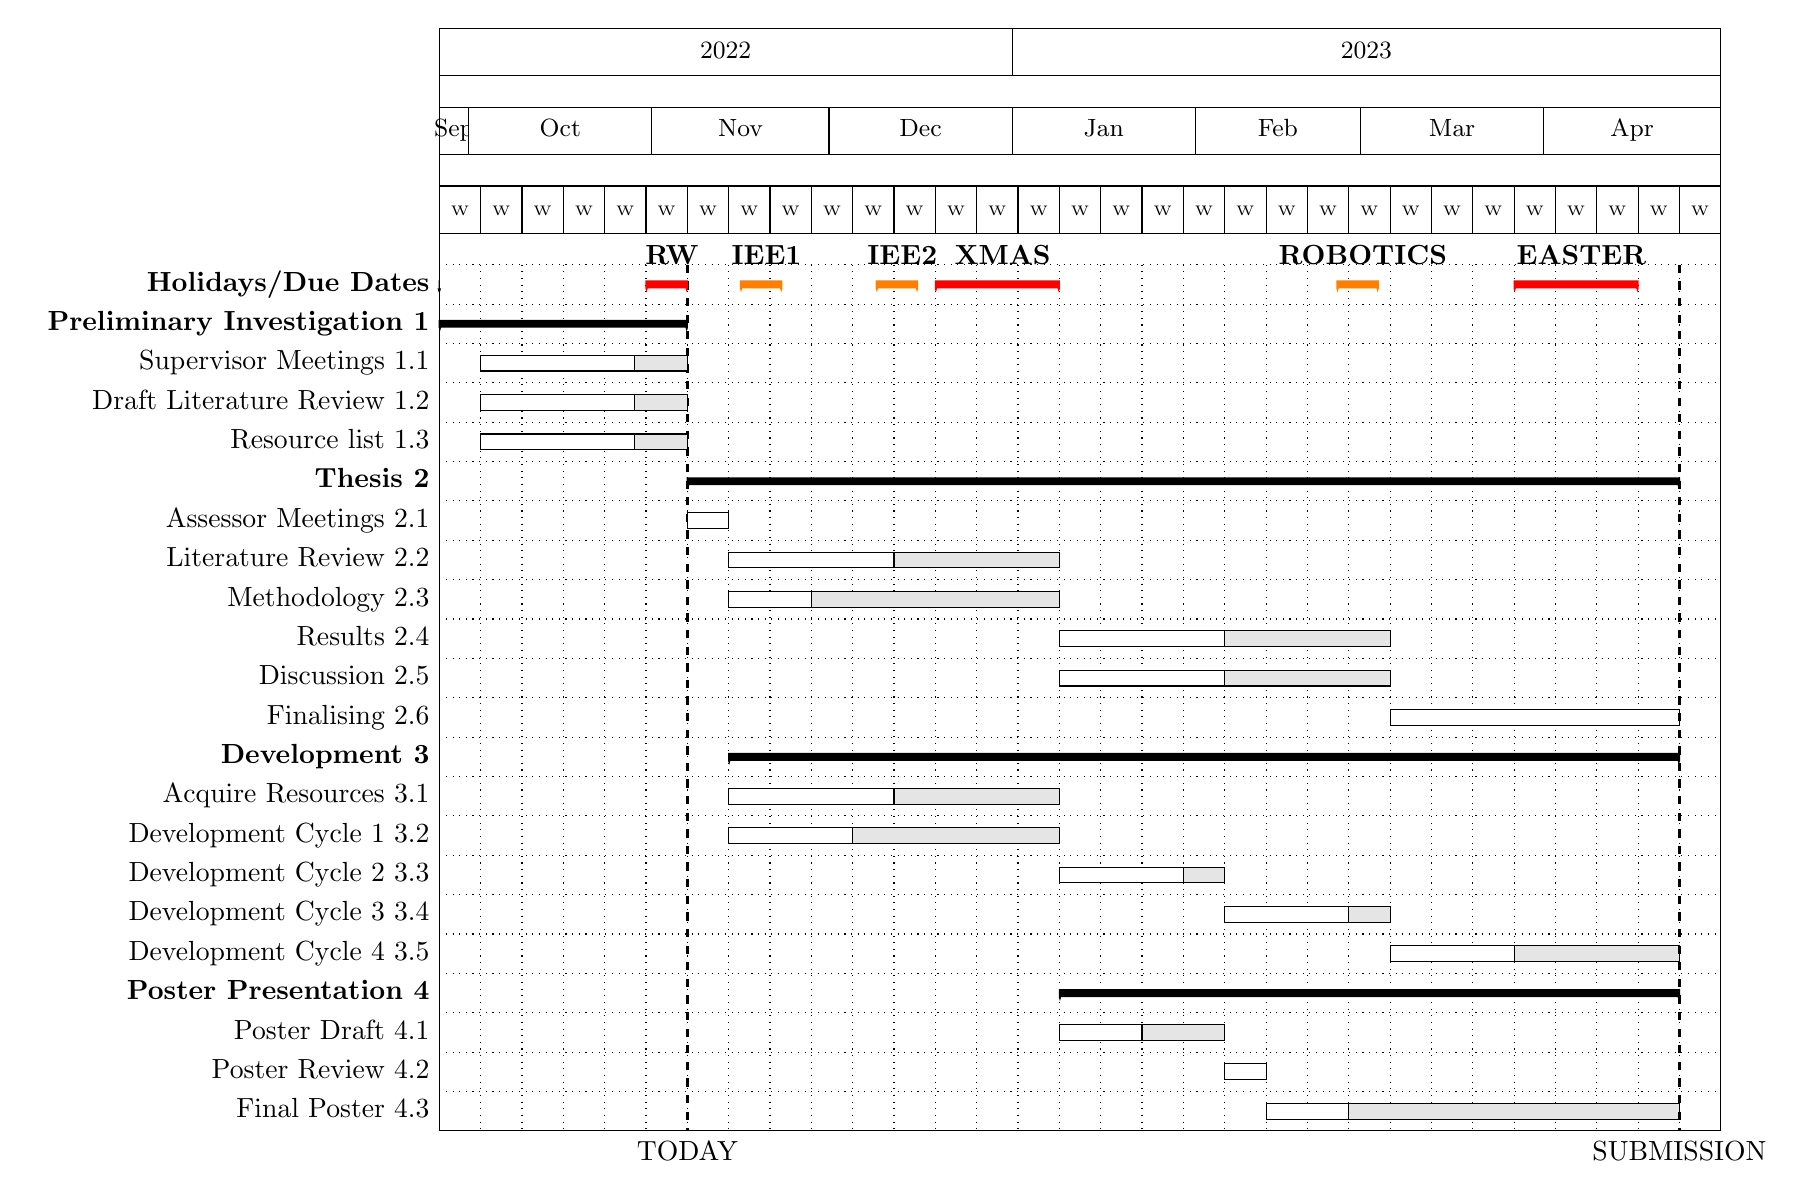
\begin{tikzpicture}

    \begin{ganttchart}[
        hgrid,
        vgrid={*6{draw=none},dotted},
        newline shortcut=true,
        x unit=.75mm,
        y unit chart=5mm,
        time slot format=isodate,
        time slot unit=day,
        group label font=\bfseries,
        % bar label font=,
        calendar week text=\tiny{W\myweek{}},
        % today=\the\year-\the\month-\the\day
        today=2022-11-06
      ]{2022-09-26}{2023-04-30}
      \gantttitlecalendar{year, month=shortname, week} \\
      
      \ganttgroup[]{Holidays/Due Dates}{2022-09-26}{2022-09-25}
      \ganttgroup[
        inline=true,
        group/.append style={fill=red},
        name=MRW]{
        RW}{2022-10-31}{2022-11-06}
      \ganttgroup[
        inline=true,
        group/.append style={fill=red},
        name=MXMS]{
        XMAS}{2022-12-19}{2023-01-08}
      \ganttgroup[
        inline=true,
        group/.append style={fill=red},
        name=MEST]{
        EASTER}{2023-03-27}{2023-04-16}
      \ganttgroup[
        inline=true,
        group/.append style={fill=orange},
        name=DIEE1]{
        IEE1}{2022-11-16}{2022-11-22}
      \ganttgroup[
        inline=true,
        group/.append style={fill=orange},
        name=DIEE2]{
        IEE2}{2022-12-09}{2022-12-15}
      \ganttgroup[
        inline=true,
        group/.append style={fill=orange},
        name=DROB]{
        ROBOTICS}{2023-02-25}{2023-03-03}
      \\
      
      \ganttgroup[name=1]{
        Preliminary Investigation 1}
      {2022-09-26}{2022-11-06} \\
      \ganttbar[bar/.append style={fill=white!90!black}]{}{2022-10-03}{2022-11-06}
      \ganttbar[name=1.1]{
        Supervisor Meetings 1.1
      }{2022-10-03}{2022-10-28}
      \\
      \ganttbar[bar/.append style={fill=white!90!black}]{}{2022-10-03}{2022-11-06}
      \ganttbar[name=1.2]{
        Draft Literature Review 1.2
      }{2022-10-03}{2022-10-28}
      \\
      \ganttbar[bar/.append style={fill=white!90!black}]{}{2022-10-03}{2022-11-06}
      \ganttbar[name=1.3]{
        Resource list 1.3
      }{2022-10-03}{2022-10-28}
      \\
      
      \ganttgroup[name=2]{
        Thesis 2}
      {2022-11-07}{2023-04-23}
      \\
      \ganttbar[name=2.1]{
        Assessor Meetings 2.1
      }{2022-11-07}{2022-11-13} \\
      \ganttbar[bar/.append style={fill=white!90!black}]{}{2022-11-14}{2023-01-08}
      \ganttbar[name=2.2]{
        Literature Review 2.2
      }{2022-11-14}{2022-12-11} \\
      \ganttbar[bar/.append style={fill=white!90!black}]{}{2022-11-14}{2023-01-08}
      \ganttbar[name=2.3]{
        Methodology 2.3
      }{2022-11-14}{2022-11-27} \\
      \ganttbar[bar/.append style={fill=white!90!black}]{}{2023-01-09}{2023-03-05}
      \ganttbar[name=2.4]{
        Results 2.4
      }{2023-01-09}{2023-02-05} \\
      \ganttbar[bar/.append style={fill=white!90!black}]{}{2023-01-09}{2023-03-05}
      \ganttbar[name=2.5]{
        Discussion 2.5
      }{2023-01-09}{2023-02-05} \\
      \ganttbar[bar/.append style={fill=white!90!black}]{}{2023-03-06}{2023-04-23}
      \ganttbar[name=2.6]{
        Finalising 2.6
      }{2023-03-06}{2023-04-23} \\
      
      \ganttgroup[name=3]{
        Development 3}
      {2022-11-14}{2023-04-23} \\
      \ganttbar[bar/.append style={fill=white!90!black}]{}{2022-11-14}{2023-01-08}
      \ganttbar[name=3.1]{
        Acquire Resources 3.1 
      }{2022-11-14}{2022-12-11} \\
      \ganttbar[bar/.append style={fill=white!90!black}]{}{2022-11-14}{2023-01-08}
      \ganttbar[name=3.2]{
        Development Cycle 1 3.2 
      }{2022-11-14}{2022-12-04} \\
      \ganttbar[bar/.append style={fill=white!90!black}]{}{2023-01-09}{2023-02-05}
      \ganttbar[name=3.3]{
        Development Cycle 2 3.3 
      }{2023-01-09}{2023-01-29} \\
      \ganttbar[bar/.append style={fill=white!90!black}]{}{2023-02-06}{2023-03-05}
      \ganttbar[name=3.4]{
        Development Cycle 3 3.4 
      }{2023-02-06}{2023-02-26} \\
      \ganttbar[bar/.append style={fill=white!90!black}]{}{2023-03-06}{2023-04-23}
      \ganttbar[name=3.5]{
        Development Cycle 4 3.5 
      }{2023-03-06}{2023-03-26} \\
      
      \ganttgroup[name=4]{
        Poster Presentation 4}
      {2023-01-09}{2023-04-23} \\
      \ganttbar[bar/.append style={fill=white!90!black}]{}{2023-01-09}{2023-02-05}
      \ganttbar[name=4.1]{
        Poster Draft 4.1 
      }{2023-01-09}{2023-01-22} \\
      % \ganttbar[bar/.append style={fill=white!90!black}]{}{2023-01-09}{2023-01-25}
      \ganttbar[name=4.2]{
        Poster Review 4.2 
      }{2023-02-06}{2023-02-12} \\
      \ganttbar[bar/.append style={fill=white!90!black}]{}{2023-02-13}{2023-04-23}
      \ganttbar[name=4.3]{
        Final Poster 4.3 
      }{2023-02-13}{2023-02-26}
      
      \ganttvrule{SUBMISSION}{2023-04-23}
      
    \end{ganttchart}
  \end{tikzpicture}
  \caption{The project work plan}
  \label{fig:The project work plan}
\end{sidewaysfigure}
% \end{landscape}
\restoregeometry

% \newgeometry{top=1cm,bottom=1cm}
% \begin{landscape}


\pagebreak
\bibliographystyle{IEEEtran}
\bibliography{ProjectSpecificationForm}

\end{document}